% !TEX encoding = UTF-8 Unicode
%!TEX root = thesis.tex
% !TEX spellcheck = en-US
%%=========================================
\section{Experiment 5}

\subsection{Configuration}
This experiment is about combining several audio effects in serial and parallel. The idea is that this allows for altering the sound in more ways than with only a single audio effect. This may yield improvements in fitness compared to using a single audio effect. The hypothesis is that the genetic algorithm could be adept at choosing what effects to use and how to combine them. This experiment will study two different effect networks, illustrated by figure \ref{fig:exp5_1layer_flow} and \ref{fig:exp5_2layers_flow}. From now on, these two configurations will be referred to as ``1 layer'' and ``2 layers'', respectively. To find out how well these effect networks perform, they will be compared to runs with individual audio effects.

The effect mix values in one layer are determined by the output of the softmax function \eqref{eq:softmax}, also called the normalized exponential function. This makes the sum of effect mixes in one layer equal to one. It also lets the neural network easily ``choose'' one single audio effect to dominate at any given time, but mixing multiple audio effects is also within reach.

\begin{equation} \label{eq:softmax}
softmax_i(a)=\frac{\exp{a_i}}{\sum\exp{a_i}}
\end{equation}

\begin{figure}[H]
    \centering
    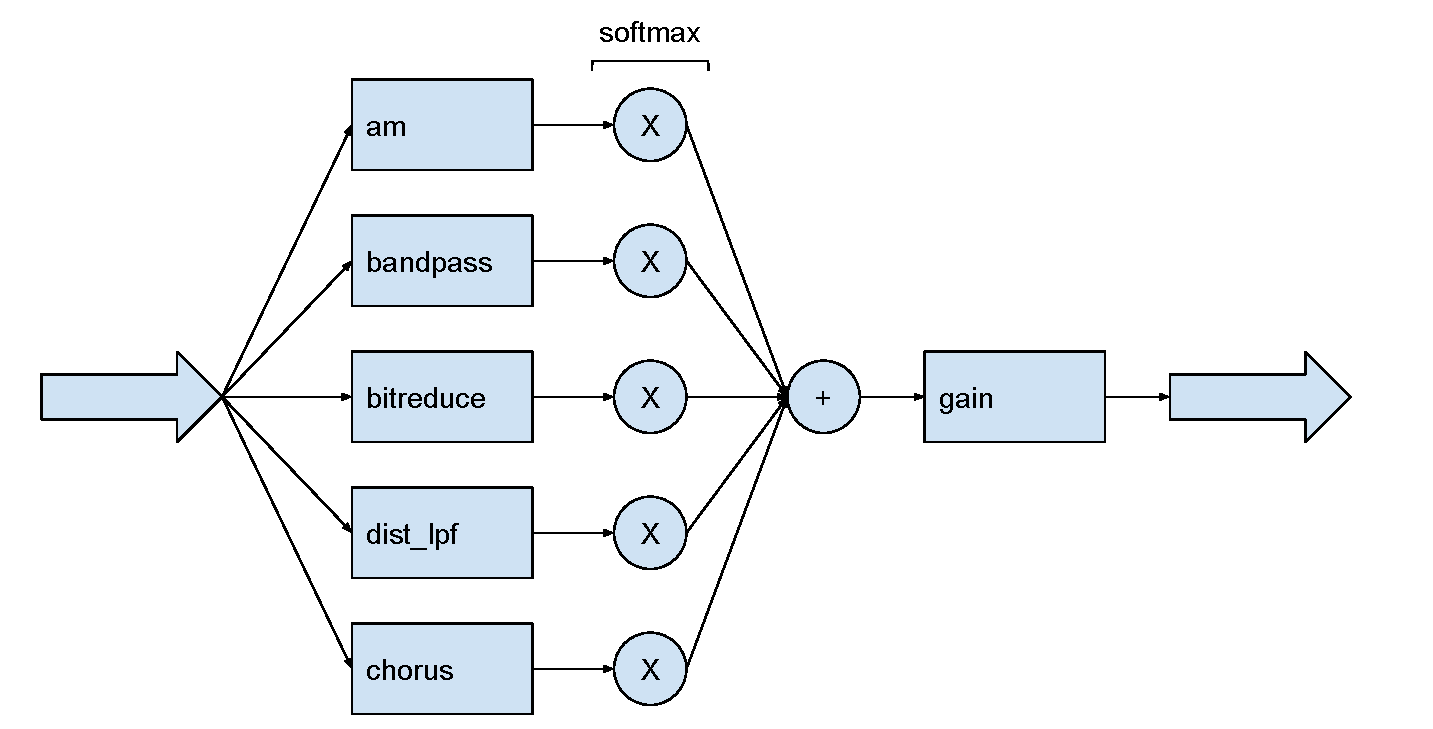
\includegraphics[width=0.75\textwidth]{exp5_1layer_flow}
    \caption{Signal flow in the ``1 layer'' configuration}
    \label{fig:exp5_1layer_flow}
\end{figure}

\begin{figure}[H]
    \centering
    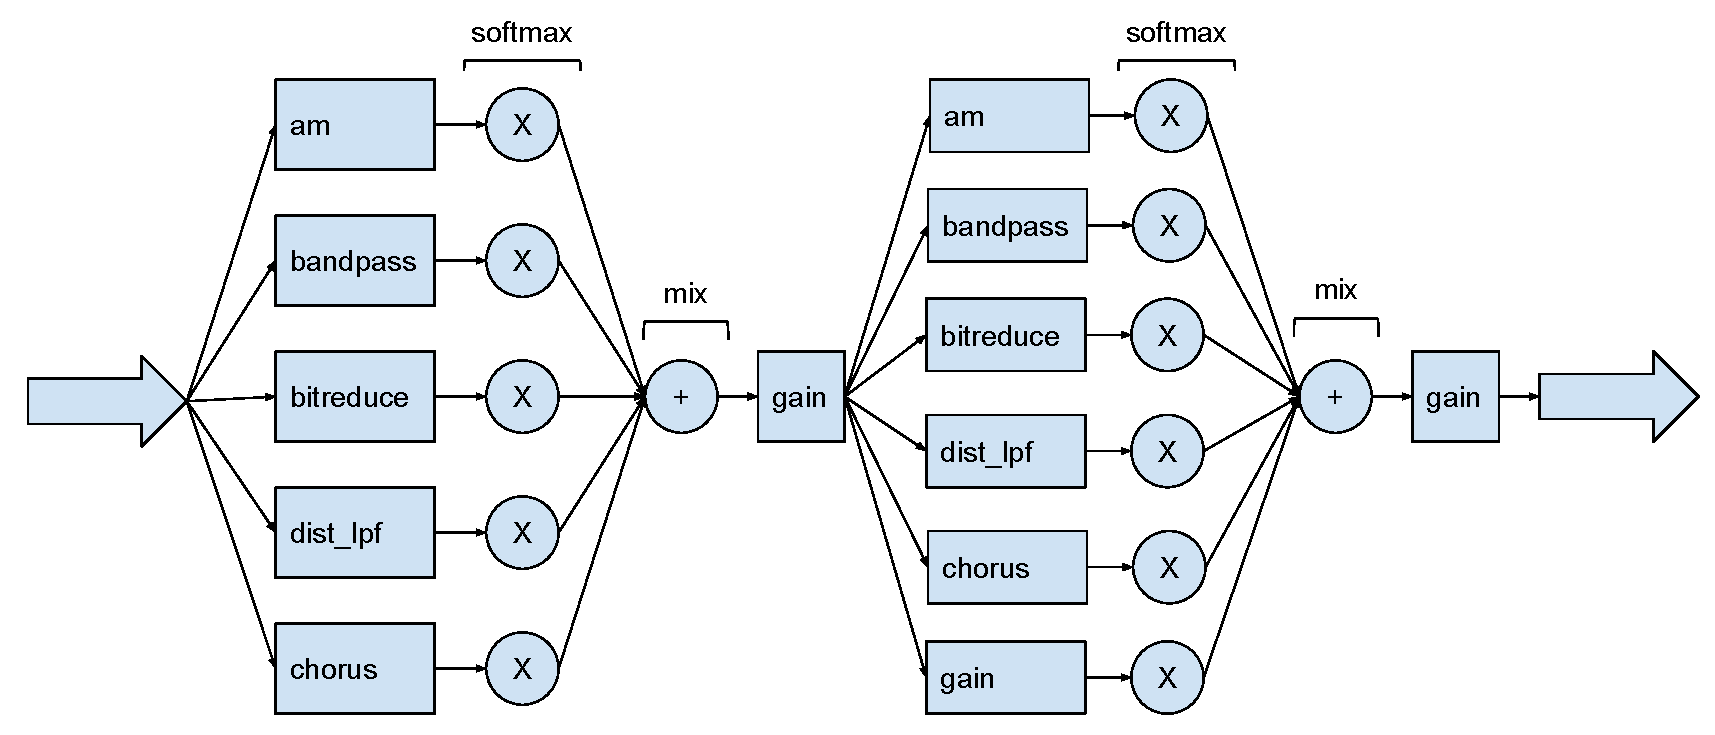
\includegraphics[width=1.0\textwidth]{exp5_2layers_flow}
    \caption{Signal flow in the ``2 layers'' configuration}
    \label{fig:exp5_2layers_flow}
\end{figure}

\begin{center}
\begin{longtable}{p{7.2cm} p{7.5cm}}
\caption[Experiment configuration]{Experiment configuration} \label{tab:exp1_configuration} \\

\hline \multicolumn{1}{l}{\textbf{Parameter}} & \multicolumn{1}{l}{\textbf{Value}} \\ \hline 
\endfirsthead

\multicolumn{2}{c}%
{{\bfseries \tablename\ \thetable{} -- continued from previous page}} \\
\hline \multicolumn{1}{l}{\textbf{Parameter}} & \multicolumn{1}{l}{\textbf{Value}} \\ \hline 
\endhead

\hline \multicolumn{2}{r}{{Continued on next page}} \\ \hline
\endfoot

\hline \hline
\endlastfoot

Number of generations & 500 \\
\midrule
Population size & 40 \\
\midrule
Target sound & Drum loop \\
\midrule
Input sound & White noise \\
\midrule
Audio features for neural input & mfcc\_0, mfcc\_0\_\_derivative, mfcc\_1 \\
\midrule
Audio features for similarity measure & mfcc\_0, mfcc\_0\_\_derivative, mfcc\_1 and bark bands \\
\midrule
Number of runs & 20 per configuration \\
\end{longtable}
\end{center}


\subsection{Results and evaluation}

\begin{figure}[H]
    \centering
    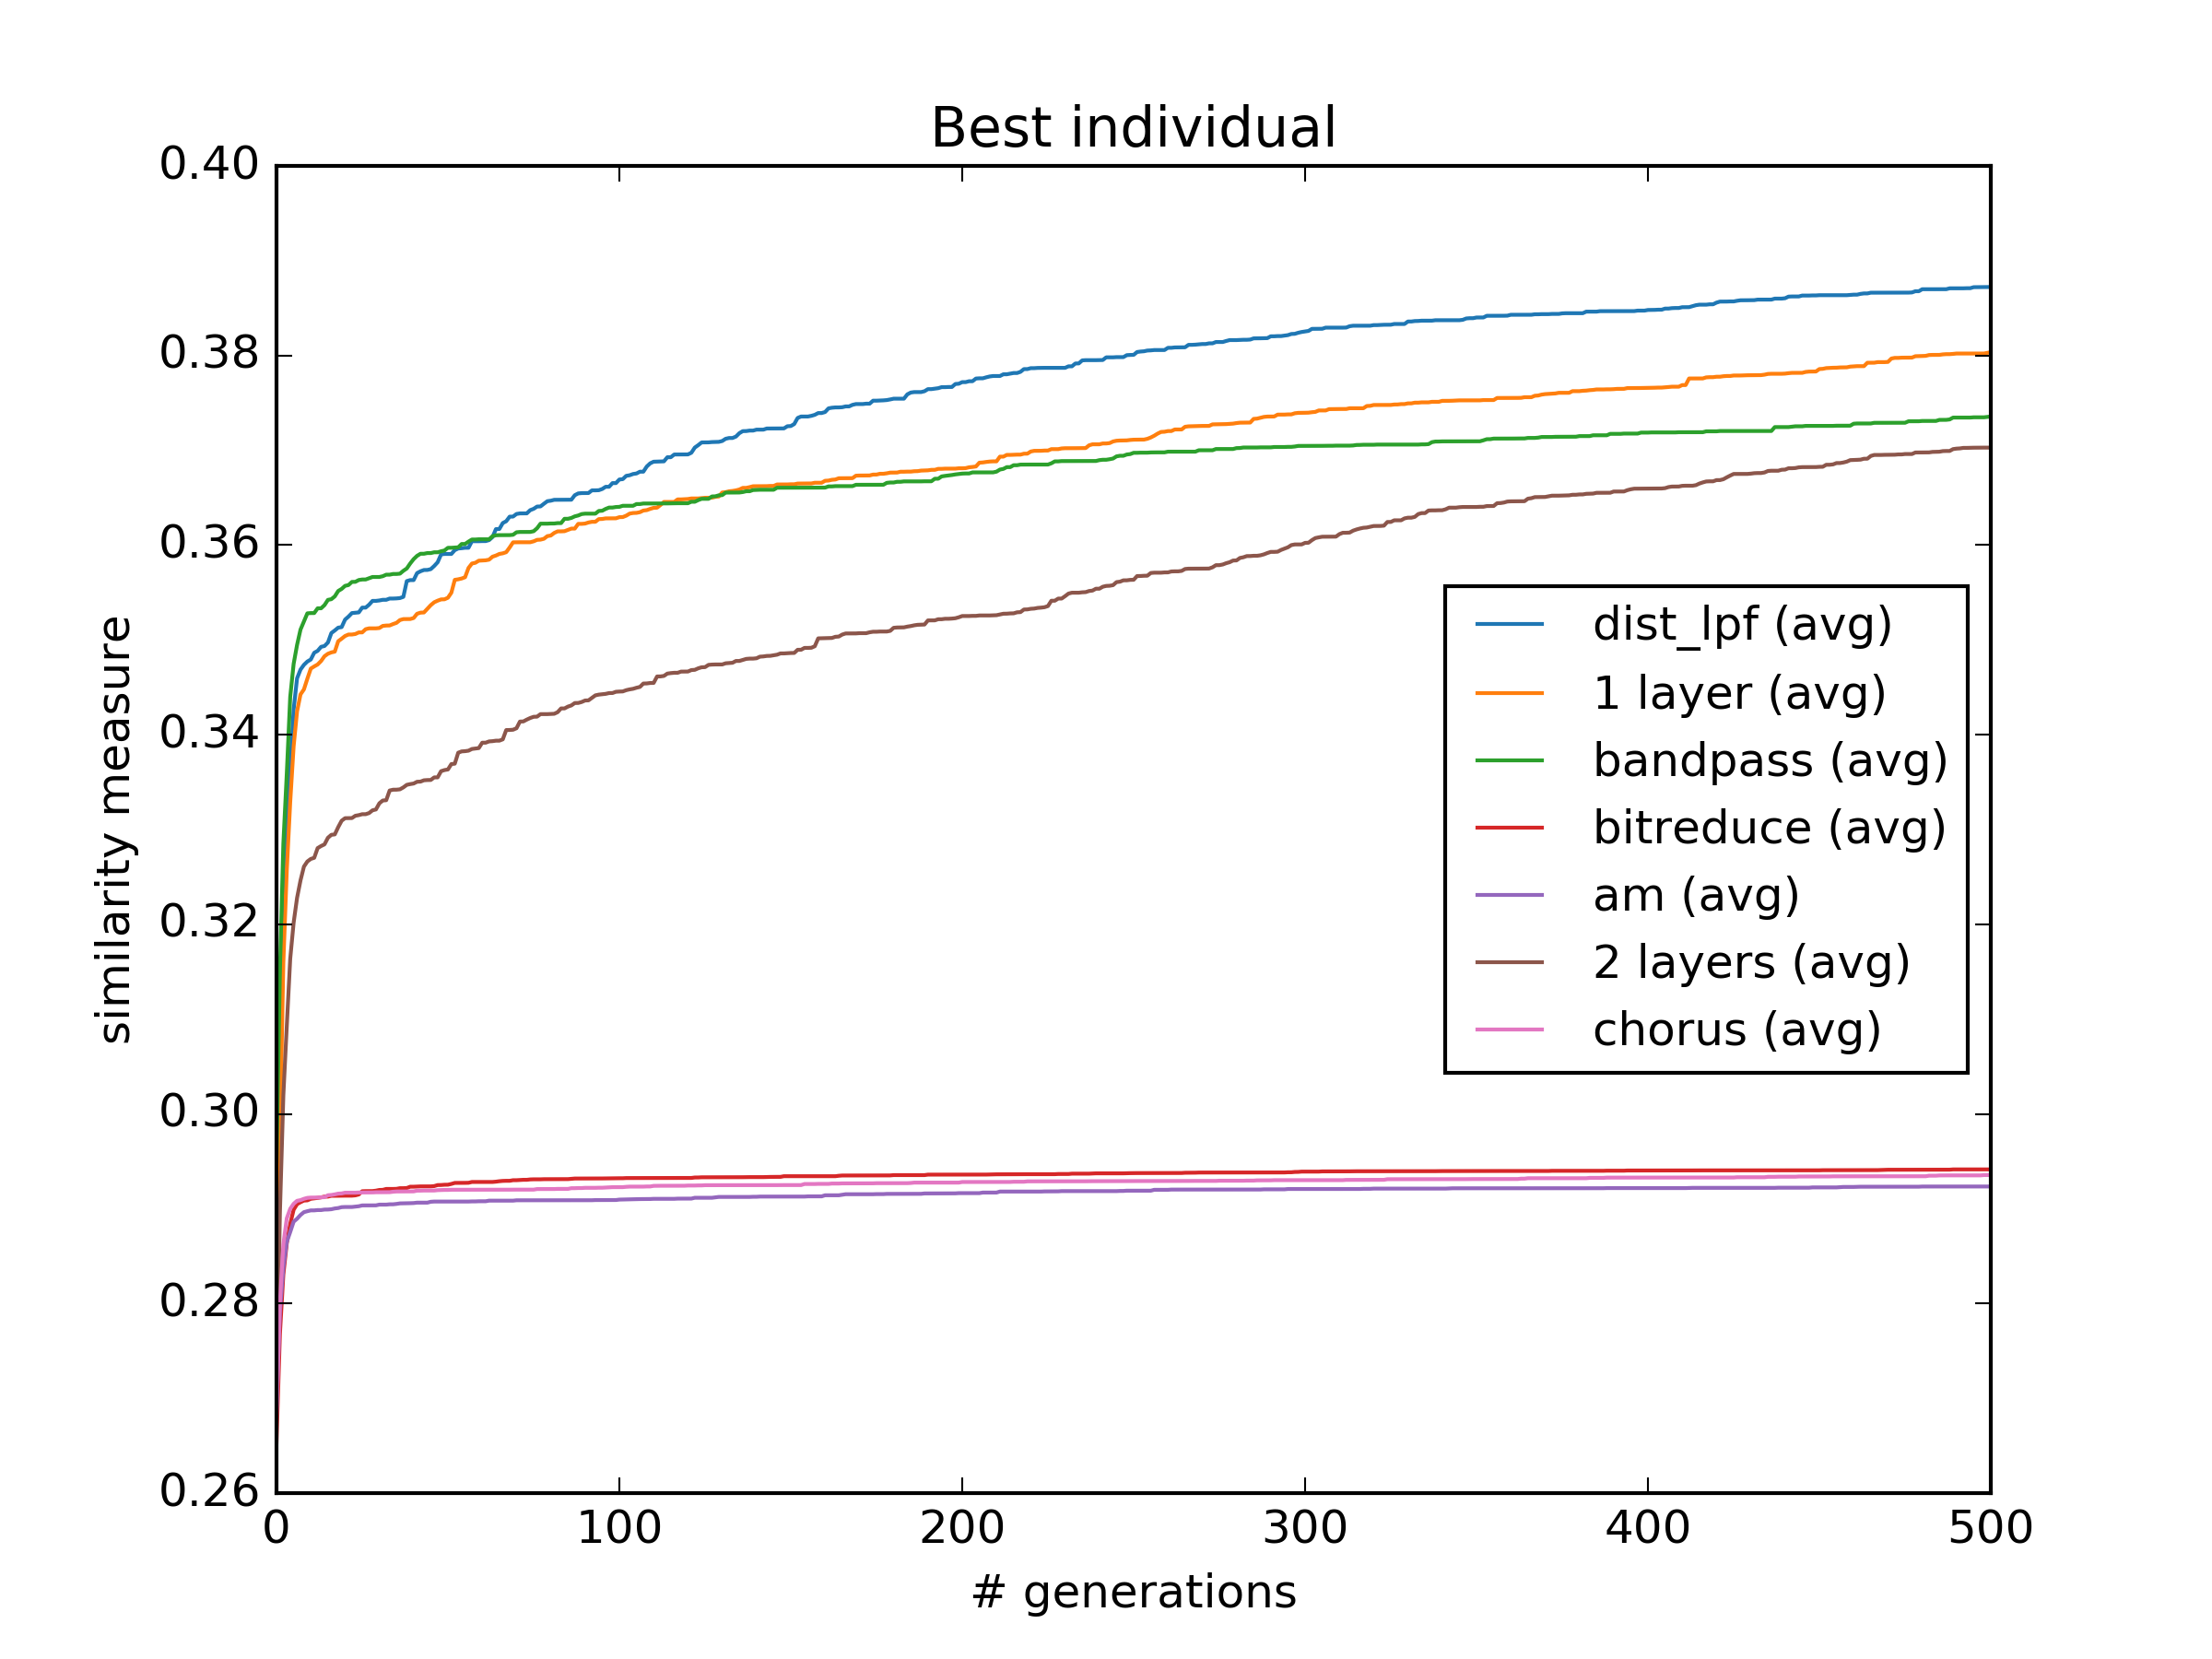
\includegraphics[width=1.0\textwidth]{exp5_avg}
    \caption{Aggregated fitness values}
    \label{fig:exp5_avg}
\end{figure}

\begin{figure}[H]
    \centering
    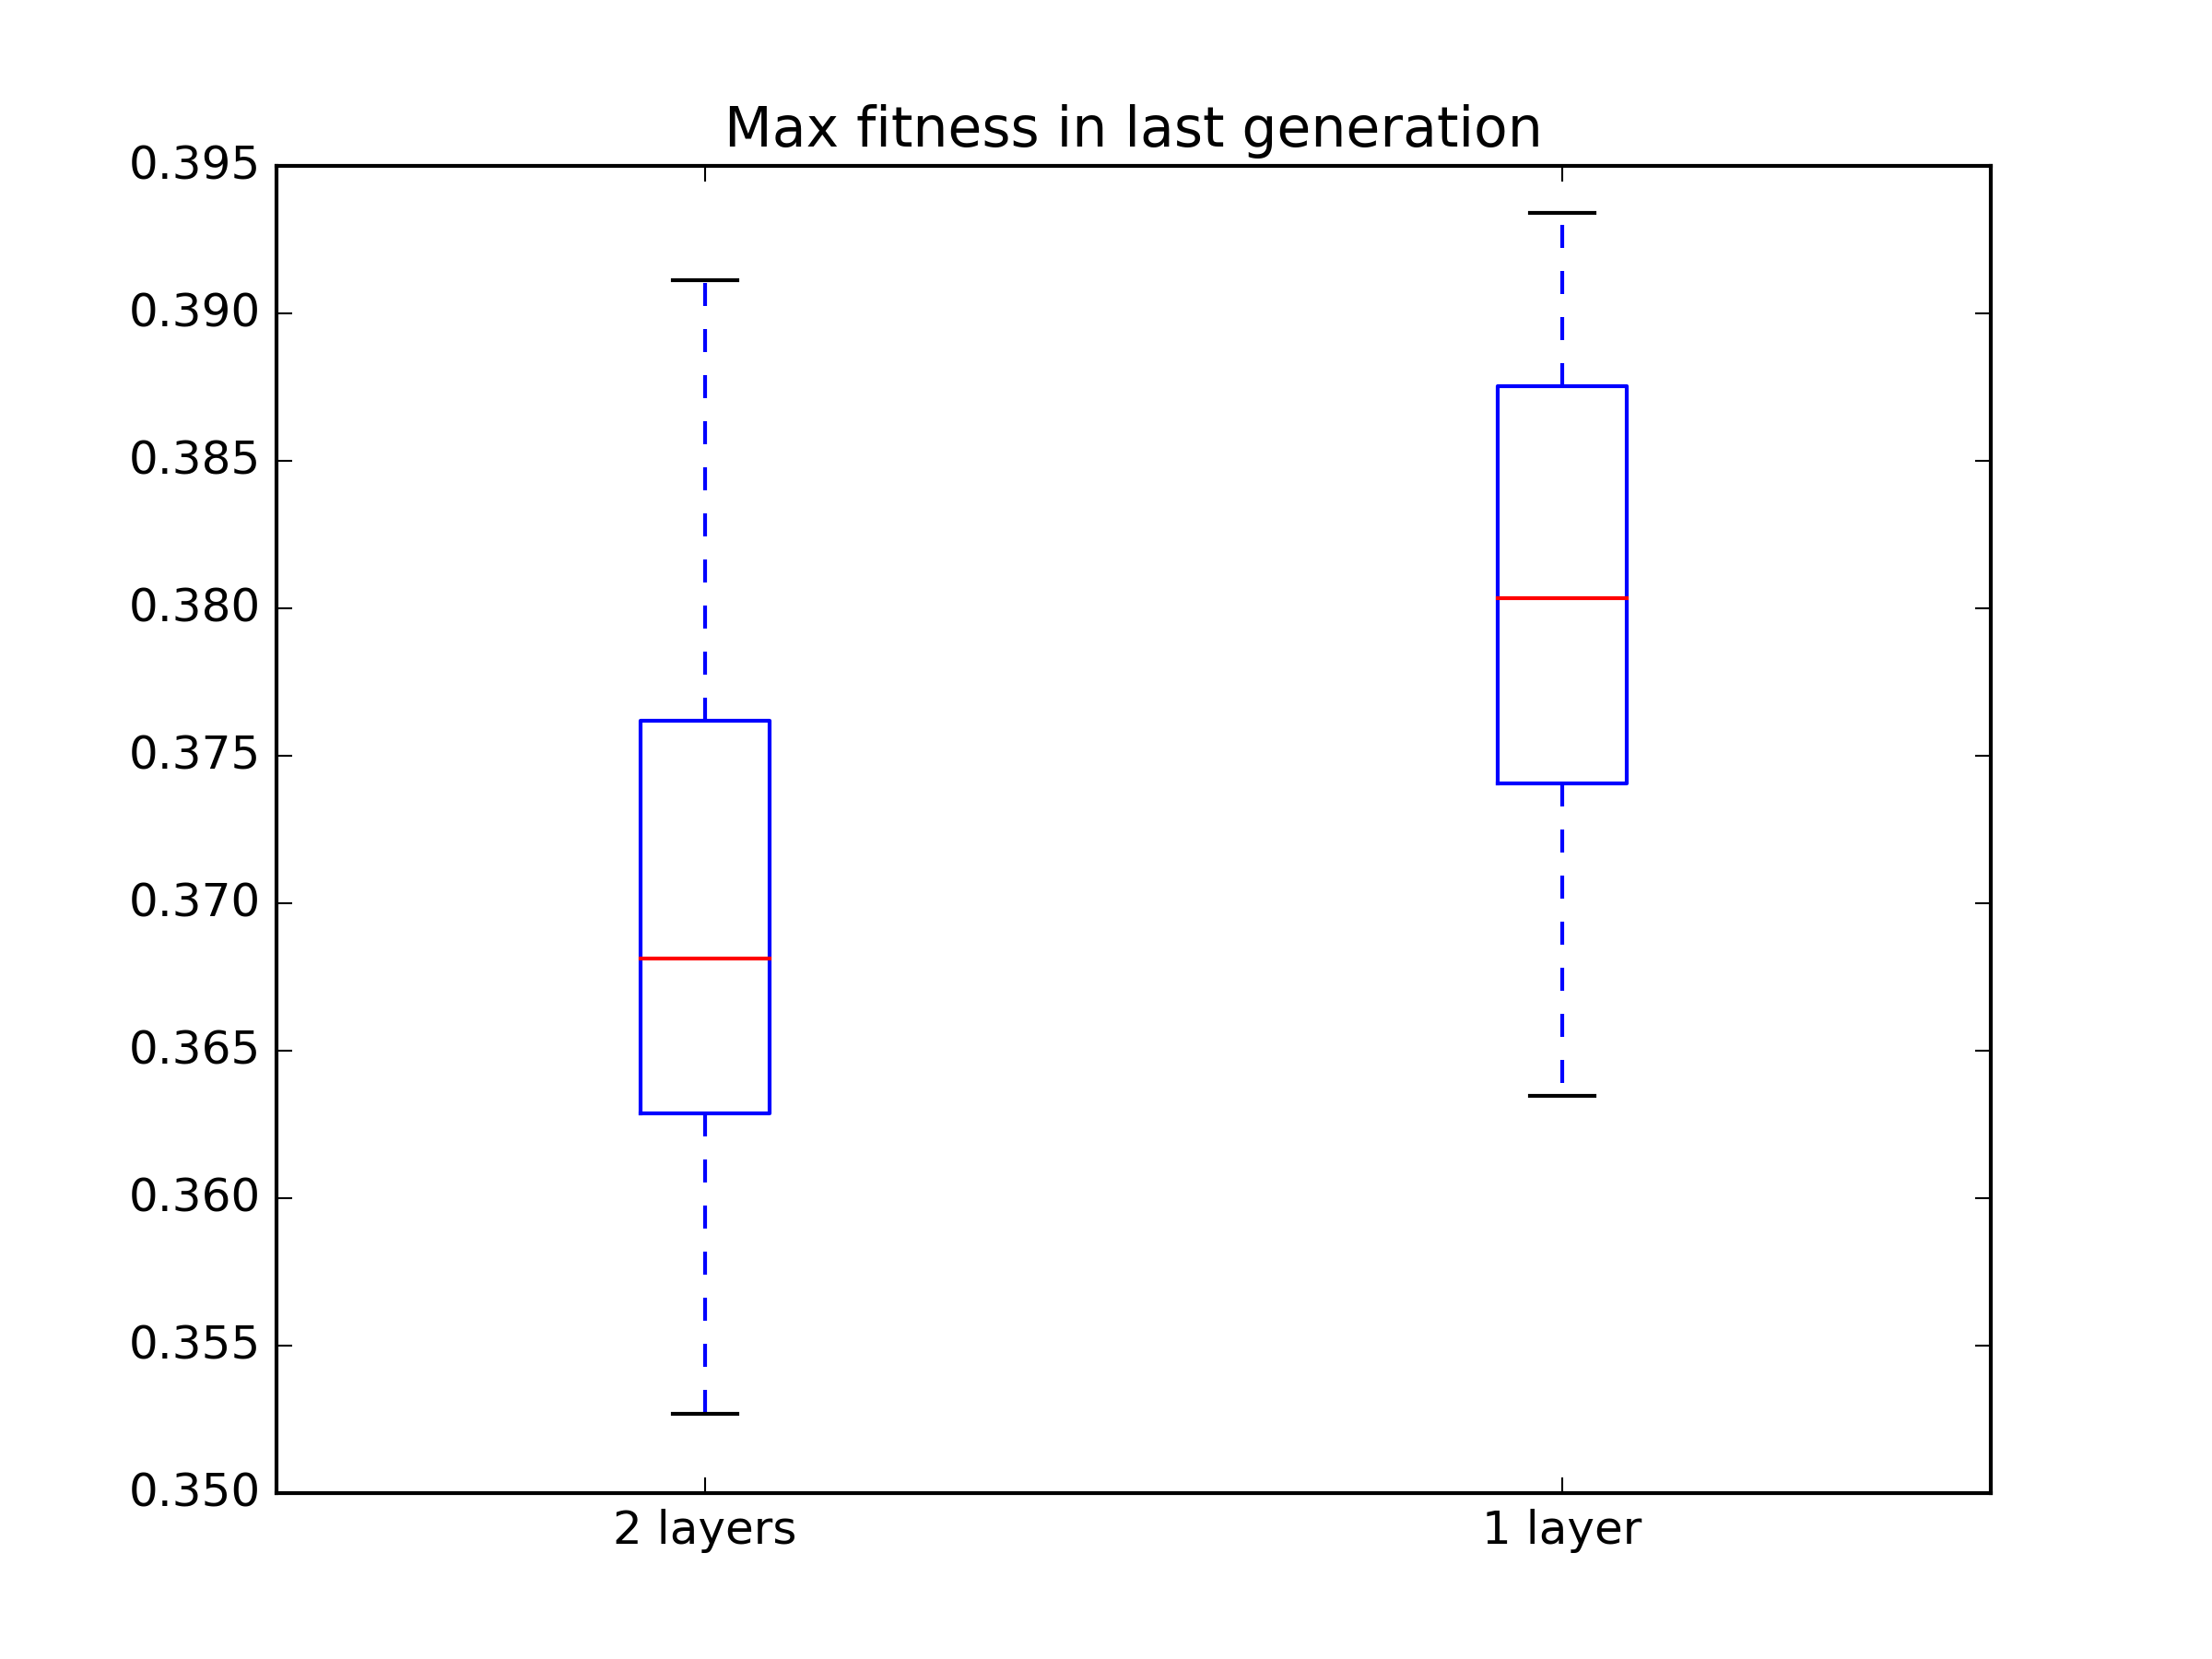
\includegraphics[width=1.0\textwidth]{exp5_box}
    \caption{Box-and-whisker plot of fitness values in the last generation}
    \label{fig:exp5_box}
\end{figure}

As illustrated by figure \ref{fig:exp5_avg} and \ref{fig:exp5_box}, three of the audio effects (amplitude modulation, chorus and bitreduce) achieve bad scores when used individually. The reason is that they are not able to shape/filter the noise in a desirable manner. This makes sense, as these three audio effects typically make the sound ``richer''. The band-pass filter and low-pass filter are more useful in this experiment, because they can filter the wide spectrum of the input sound (white noise) to something that sounds more like the target sound (drums). Hence low mix values for am, chorus and bitreduce are expected in the ``1 layer'' and the ``2 layers'' runs. Indeed, when inspecting the mix values in the best runs, we find that bandpass and dist\_lpf are used much (see figure \ref{fig:exp5_1layer_softmax} and \ref{fig:exp5_2layers_softmax}). However, we also find that chorus and bitreduce are used for representing the snare drum (the rightmost part). In the sound illustrated by figure \ref{fig:exp5_1layer_softmax} the mix values change rapidly at one point, and this gives the snare drum a flutter-like texture and creates the illusion of a short echo. The waveform of this sound can be seen in figure \ref{fig:exp5_1layer_waveform}.

While the algorithm may have found out which effects are not useful, it has not found out how to use the useful effects in a good way. Note that dist\_lpf alone yields better results than 1 layer. Theoretically, both 1 layer and 2 layers could produce solutions as good as those with dist\_lpf, but that typically does not happen, at least not with the same number of generations.

One key takeaway from this experiment is that one should only use audio effects that are known to be useful in the context of the experiments. Adding unfitting audio effects to an audio effect network makes the search space larger and has a negative impact on the convergence rate. In other words, to get good results with effect networks, let a human expert create the audio effect structure.

Here are some ideas that could be applied to improve the results of audio effect networks:

\begin{itemize}
\item Perform pre-training on the parameters of the various audio effects separately. Then freeze those neural networks and train the mix of the output from the effects when they are used in parallel.
\item The assumptions behind softmax mix values might be suboptimal. Using independent mix values, i.e. without any normalization, might yield better results.
\item Use Cartesian Genetic Programming (CGP) to automatically evolve networks of interconnected audio effects.
\end{itemize}

% TODO create video demonstrating 1st successful result here?

\begin{figure}[h]
    \centering
    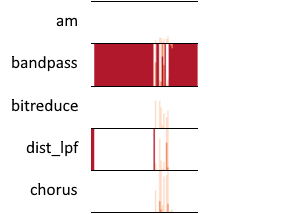
\includegraphics[width=0.45\textwidth]{exp5_1layer_softmax}
    \caption{Mix values for each effect in the best result from the runs with 1 layer}
    \label{fig:exp5_1layer_softmax}
\end{figure}

\begin{figure}[h]
    \centering
    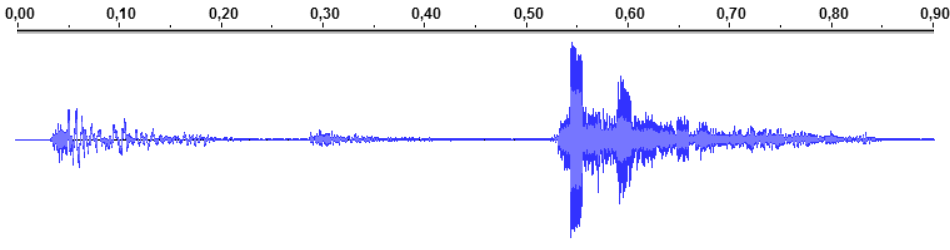
\includegraphics[width=0.95\textwidth]{exp5_1layer_waveform}
    \caption{Waveform of the best output sound from the runs with 1 layer}
    \label{fig:exp5_1layer_waveform}
\end{figure}

\begin{figure}[h]
    \centering
    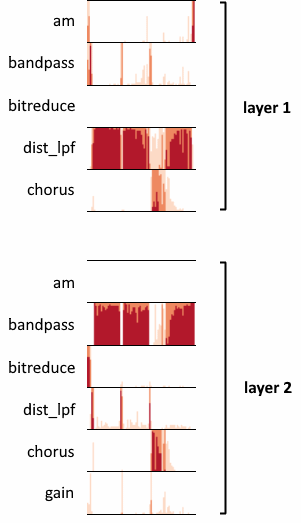
\includegraphics[width=0.45\textwidth]{exp5_2layers_softmax}
    \caption{Mix values for each effect in the best result from the runs with 2 layers}
    \label{fig:exp5_2layers_softmax}
\end{figure}
